\documentclass{article}
\usepackage{pslatex}
\usepackage{amssymb}
\pagestyle{empty}
\usepackage{graphicx}
\usepackage{grffile}
\usepackage{fullpage}
\begin{document}
\section{Morphology: data\_0.528\_3.8\_000160 }
\parbox{0.35\textwidth}{
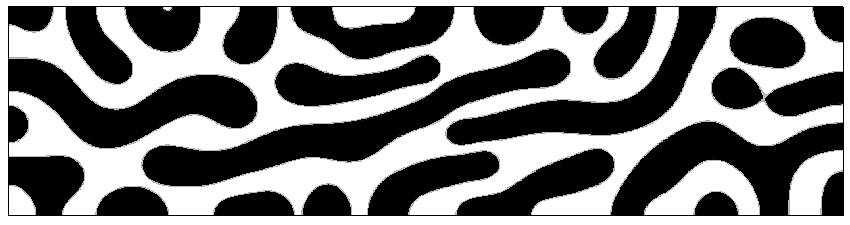
\includegraphics[width=0.35\textwidth]{/Users/owodo/MINE/PROJECTS/GraSPI/GraSPI/examples/2phaseMorphologies/thinFilm/figs/data_0.528_3.8_000160.png} \  
 ~\newline ~\newline 
\begin{small}
STAT n 40501\\
STAT e 3698\\
STAT n D 19268\\
STAT n A 21233\\
STAT CC D 22\\
STAT CC A 5\\
STAT CC D An 9\\
STAT CC A Ca 3\\
ABS wf D 0.298392\\
ABS f D 0.475741\\
DISS wf10 D 0.617915\\
DISS f10 D 0.991956\\
CT f conn D 0.665712\\
CT f e conn 0.296376\\
CT f conn D An 0.319545\\
CT f conn A Ca 0.979843\\
CT e conn 1096\\
CT e D An 1159\\
CT e A Ca 3668\\
CT f D tort1 0.522495\\
CT f A tort1 0.152944\\

DISS dist D Int $\mu$=3.49326 , $\sigma$=2.36865 \newline
CT dist Int Ca via A $\mu$=93.3219 , $\sigma$=62.6267 \newline
CT dist Int A via D $\mu$=34.1267 , $\sigma$=37.6514 \newline
\end{small}
}
\parbox{0.60\textwidth}{
\parbox{0.3\textwidth}{\centering Distance from A to Ca \newline
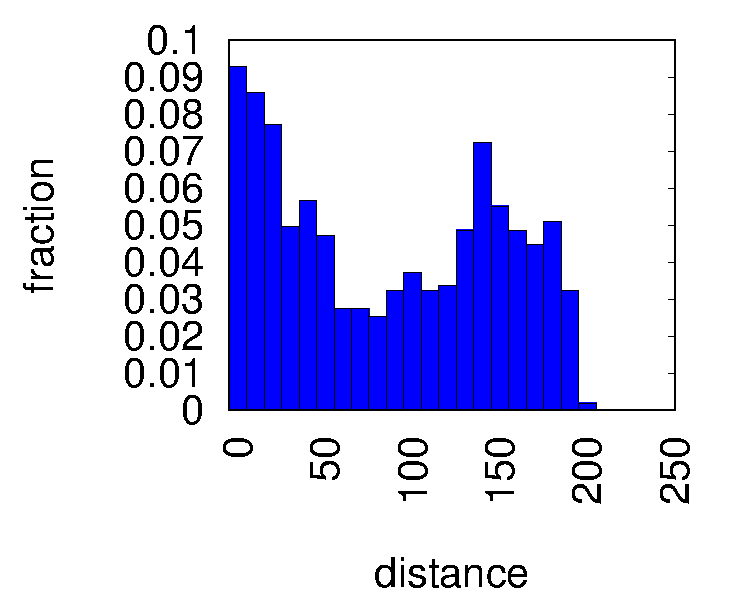
\includegraphics[width=0.3\textwidth]{/Users/owodo/MINE/PROJECTS/GraSPI/GraSPI/examples/2phaseMorphologies/thinFilm/histograms/data_0.528_3.8_000160.txtHistogramFullereneToCathode.pdf} \ ~ \ } 
\parbox{0.3\textwidth}{\centering Distance from D to Am \newline
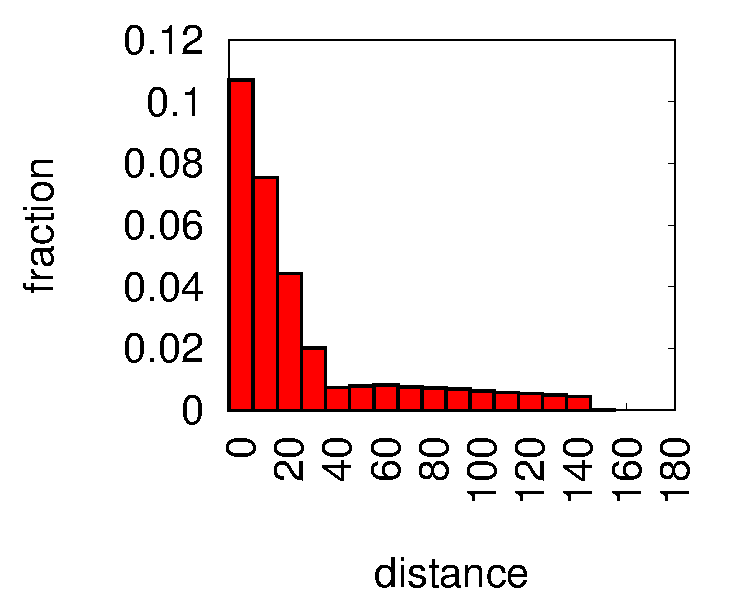
\includegraphics[width=0.3\textwidth]{/Users/owodo/MINE/PROJECTS/GraSPI/GraSPI/examples/2phaseMorphologies/thinFilm/histograms/data_0.528_3.8_000160.txtHistogramPolymerToAnode.pdf} \ ~ \ }
\parbox{0.3\textwidth}{\centering Path balance \newline 
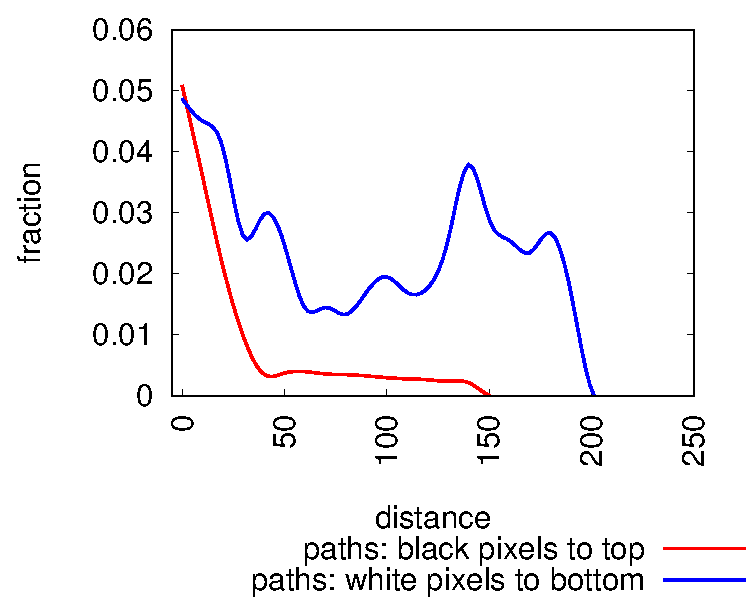
\includegraphics[width=0.3\textwidth]{/Users/owodo/MINE/PROJECTS/GraSPI/GraSPI/examples/2phaseMorphologies/thinFilm/histograms/data_0.528_3.8_000160.txtBothHistogramsUsefulDomains.pdf} \ ~ \ }
\parbox{0.3\textwidth}{\centering Distance from D to Int \newline 
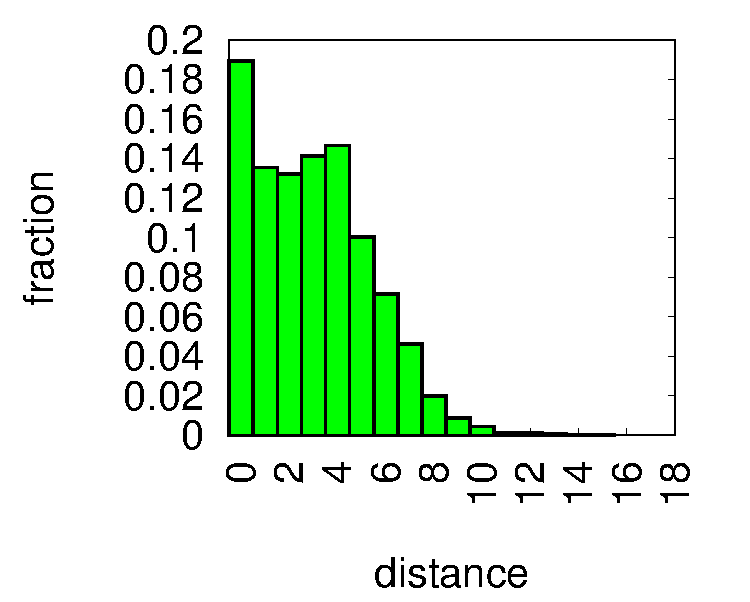
\includegraphics[width=0.3\textwidth]{/Users/owodo/MINE/PROJECTS/GraSPI/GraSPI/examples/2phaseMorphologies/thinFilm/histograms/data_0.528_3.8_000160.txtHistogramPolymerToInterface.pdf} \ ~ \ }
\parbox{0.3\textwidth}{\centering Tortuosity of D-paths to An  \newline
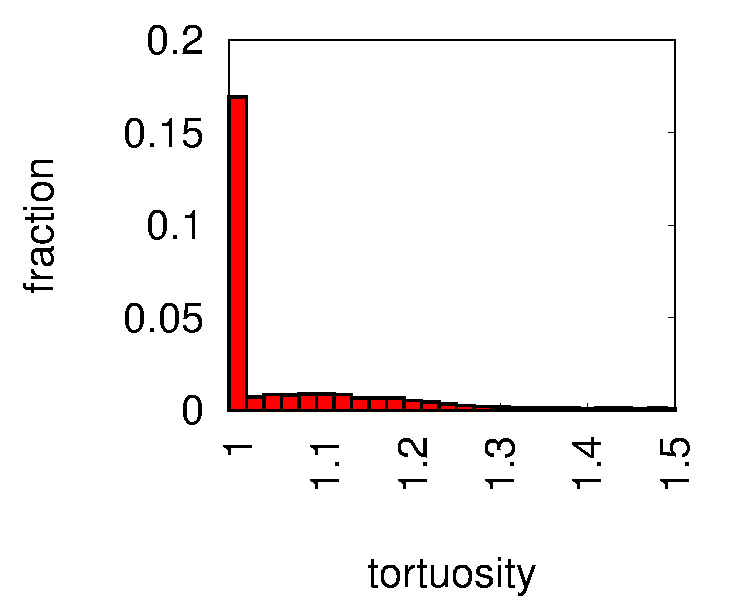
\includegraphics[width=0.3\textwidth]{/Users/owodo/MINE/PROJECTS/GraSPI/GraSPI/examples/2phaseMorphologies/thinFilm/histograms/data_0.528_3.8_000160.txtHistogramTortuosityPolymerToAnode.pdf} \ ~ \ }
\parbox{0.3\textwidth}{\centering Tortuosity of A-paths to Ca \newline
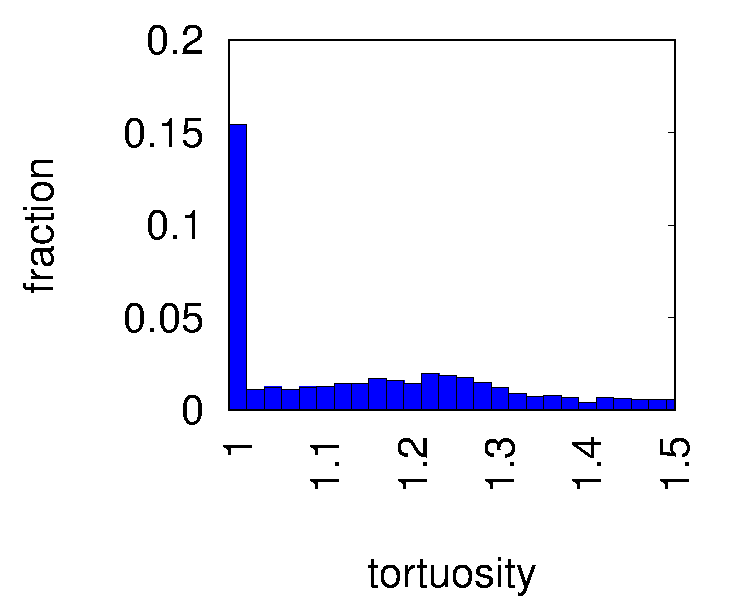
\includegraphics[width=0.3\textwidth]{/Users/owodo/MINE/PROJECTS/GraSPI/GraSPI/examples/2phaseMorphologies/thinFilm/histograms/data_0.528_3.8_000160.txtHistogramTortuosityFullereneToCathode.pdf} \ ~ \ }
}
\newpage
\section{Morphology: data\_0.5\_2.6\_000160 }
\parbox{0.35\textwidth}{
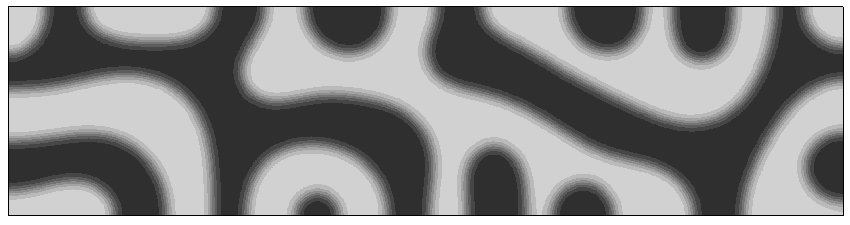
\includegraphics[width=0.35\textwidth]{/Users/owodo/MINE/PROJECTS/GraSPI/GraSPI/examples/2phaseMorphologies/thinFilm/figs/data_0.5_2.6_000160.png} \  
 ~\newline ~\newline 
\begin{small}
STAT n 40501\\
STAT e 2022\\
STAT n D 20193\\
STAT n A 20308\\
STAT CC D 8\\
STAT CC A 6\\
STAT CC D An 4\\
STAT CC A Ca 3\\
ABS wf D 0.313409\\
ABS f D 0.49858\\
DISS wf10 D 0.39619\\
DISS f10 D 0.772694\\
CT f conn D 0.767487\\
CT f e conn 0.472305\\
CT f conn D An 0.81038\\
CT f conn A Ca 0.724837\\
CT e conn 955\\
CT e D An 1558\\
CT e A Ca 1429\\
CT f D tort1 0.37167\\
CT f A tort1 0.459171\\

DISS dist D Int $\mu$=6.45987 , $\sigma$=4.1160 \newline
CT dist Int Ca via A $\mu$=47.092 , $\sigma$=36.9185 \newline
CT dist Int A via D $\mu$=53.5668 , $\sigma$=38.1929 \newline
\end{small}
}
\parbox{0.60\textwidth}{
\parbox{0.3\textwidth}{\centering Distance from A to Ca \newline
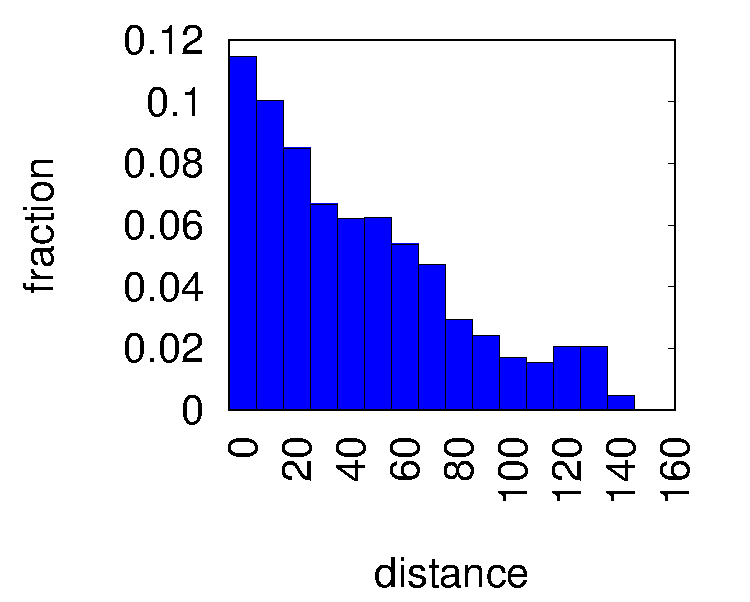
\includegraphics[width=0.3\textwidth]{/Users/owodo/MINE/PROJECTS/GraSPI/GraSPI/examples/2phaseMorphologies/thinFilm/histograms/data_0.5_2.6_000160.txtHistogramFullereneToCathode.pdf} \ ~ \ } 
\parbox{0.3\textwidth}{\centering Distance from D to Am \newline
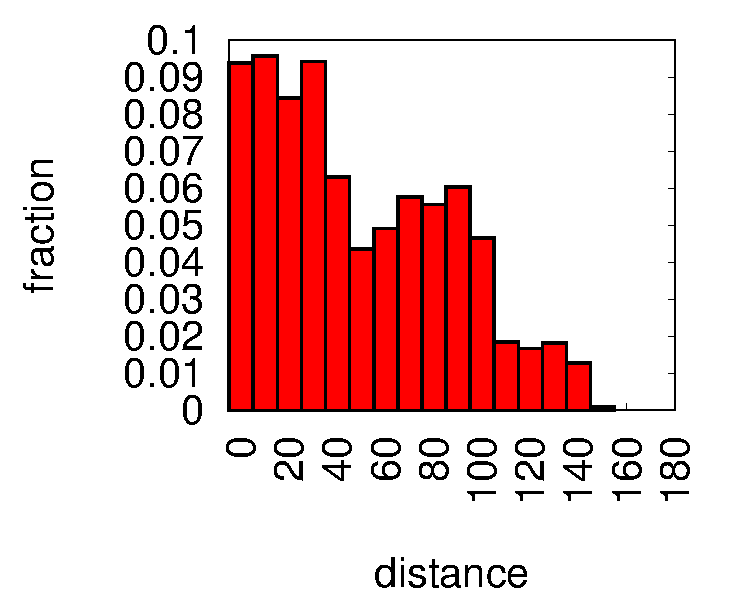
\includegraphics[width=0.3\textwidth]{/Users/owodo/MINE/PROJECTS/GraSPI/GraSPI/examples/2phaseMorphologies/thinFilm/histograms/data_0.5_2.6_000160.txtHistogramPolymerToAnode.pdf} \ ~ \ }
\parbox{0.3\textwidth}{\centering Path balance \newline 
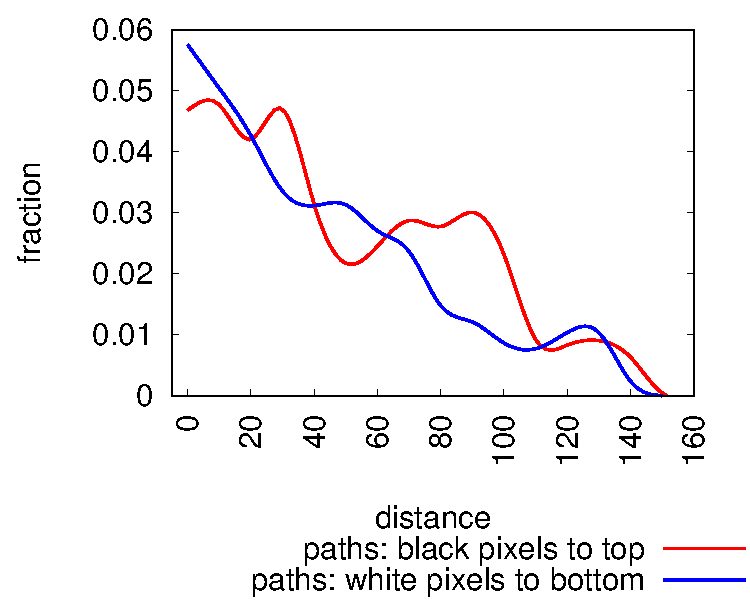
\includegraphics[width=0.3\textwidth]{/Users/owodo/MINE/PROJECTS/GraSPI/GraSPI/examples/2phaseMorphologies/thinFilm/histograms/data_0.5_2.6_000160.txtBothHistogramsUsefulDomains.pdf} \ ~ \ }
\parbox{0.3\textwidth}{\centering Distance from D to Int \newline 
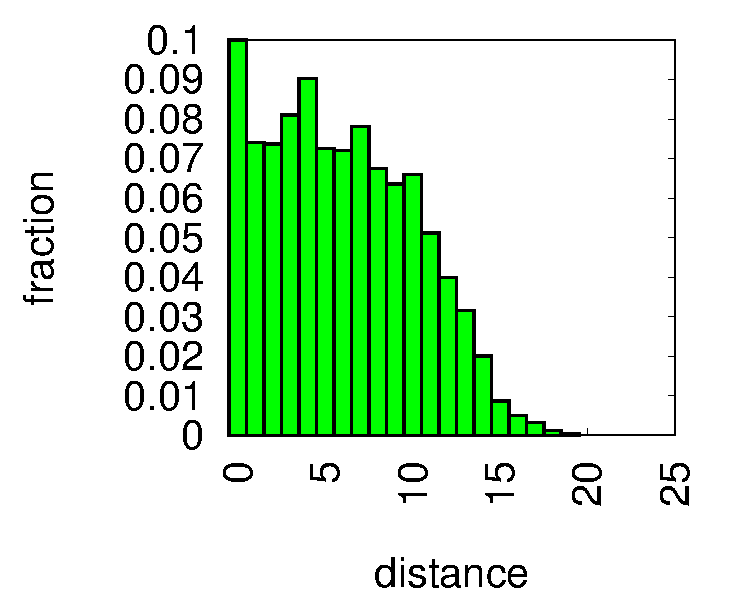
\includegraphics[width=0.3\textwidth]{/Users/owodo/MINE/PROJECTS/GraSPI/GraSPI/examples/2phaseMorphologies/thinFilm/histograms/data_0.5_2.6_000160.txtHistogramPolymerToInterface.pdf} \ ~ \ }
\parbox{0.3\textwidth}{\centering Tortuosity of D-paths to An  \newline
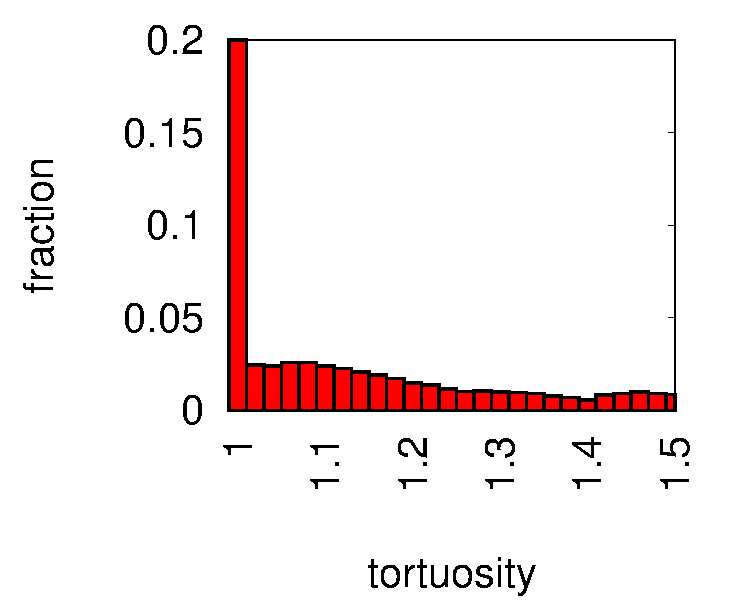
\includegraphics[width=0.3\textwidth]{/Users/owodo/MINE/PROJECTS/GraSPI/GraSPI/examples/2phaseMorphologies/thinFilm/histograms/data_0.5_2.6_000160.txtHistogramTortuosityPolymerToAnode.pdf} \ ~ \ }
\parbox{0.3\textwidth}{\centering Tortuosity of A-paths to Ca \newline
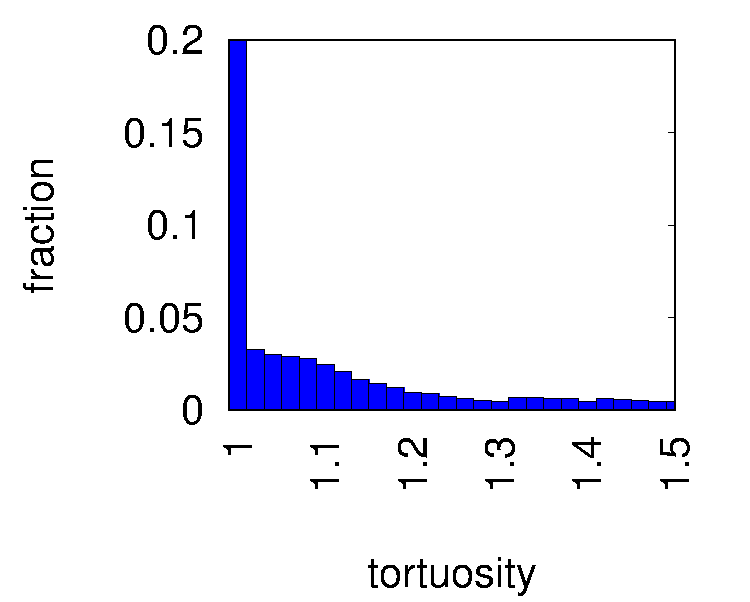
\includegraphics[width=0.3\textwidth]{/Users/owodo/MINE/PROJECTS/GraSPI/GraSPI/examples/2phaseMorphologies/thinFilm/histograms/data_0.5_2.6_000160.txtHistogramTortuosityFullereneToCathode.pdf} \ ~ \ }
}
\newpage
\section{Morphology: data\_0.615\_4.0\_000160 }
\parbox{0.35\textwidth}{
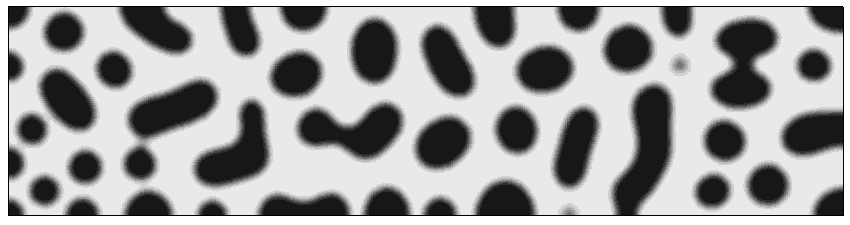
\includegraphics[width=0.35\textwidth]{/Users/owodo/MINE/PROJECTS/GraSPI/GraSPI/examples/2phaseMorphologies/thinFilm/figs/data_0.615_4.0_000160.png} \  
 ~\newline ~\newline 
\begin{small}
STAT n 40501\\
STAT e 3523\\
STAT n D 16223\\
STAT n A 24278\\
STAT CC D 43\\
STAT CC A 1\\
STAT CC D An 7\\
STAT CC A Ca 1\\
ABS wf D 0.25068\\
ABS f D 0.400558\\
DISS wf10 D 0.610803\\
DISS f10 D 0.988843\\
CT f conn D 0.653194\\
CT f e conn 0.123474\\
CT f conn D An 0.134192\\
CT f conn A Ca 1\\
CT e conn 435\\
CT e D An 419\\
CT e A Ca 3658\\
CT f D tort1 0.890216\\
CT f A tort1 0.265837\\

DISS dist D Int $\mu$=3.63377 , $\sigma$=2.61406 \newline
CT dist Int Ca via A $\mu$=53.4624 , $\sigma$=30.9465 \newline
CT dist Int A via D $\mu$=10.7625 , $\sigma$=6.6289 \newline
\end{small}
}
\parbox{0.60\textwidth}{
\parbox{0.3\textwidth}{\centering Distance from A to Ca \newline
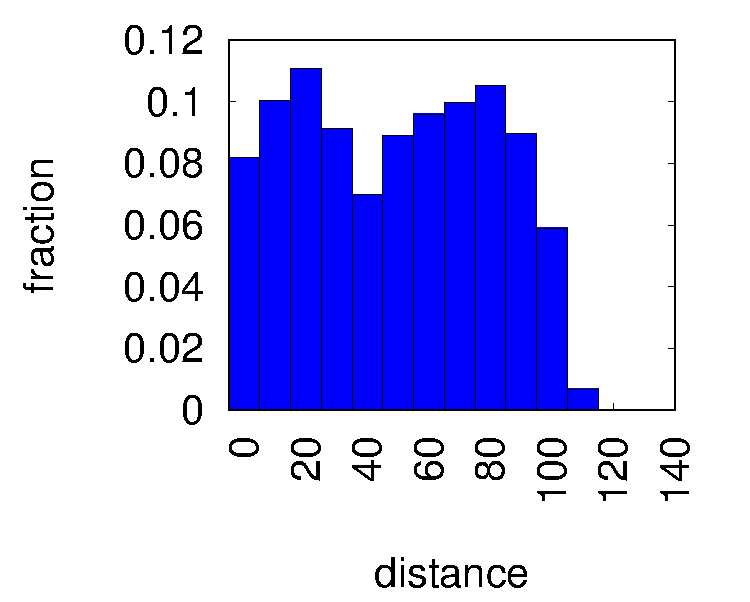
\includegraphics[width=0.3\textwidth]{/Users/owodo/MINE/PROJECTS/GraSPI/GraSPI/examples/2phaseMorphologies/thinFilm/histograms/data_0.615_4.0_000160.txtHistogramFullereneToCathode.pdf} \ ~ \ } 
\parbox{0.3\textwidth}{\centering Distance from D to Am \newline
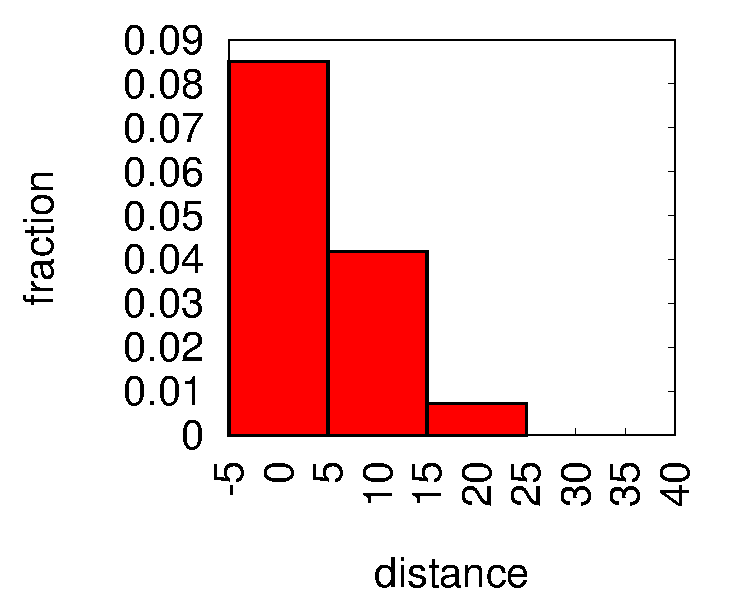
\includegraphics[width=0.3\textwidth]{/Users/owodo/MINE/PROJECTS/GraSPI/GraSPI/examples/2phaseMorphologies/thinFilm/histograms/data_0.615_4.0_000160.txtHistogramPolymerToAnode.pdf} \ ~ \ }
\parbox{0.3\textwidth}{\centering Path balance \newline 
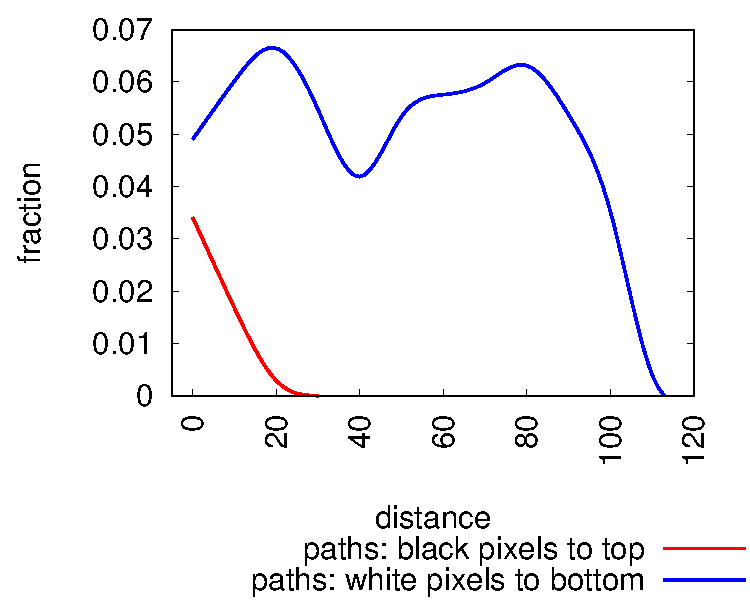
\includegraphics[width=0.3\textwidth]{/Users/owodo/MINE/PROJECTS/GraSPI/GraSPI/examples/2phaseMorphologies/thinFilm/histograms/data_0.615_4.0_000160.txtBothHistogramsUsefulDomains.pdf} \ ~ \ }
\parbox{0.3\textwidth}{\centering Distance from D to Int \newline 
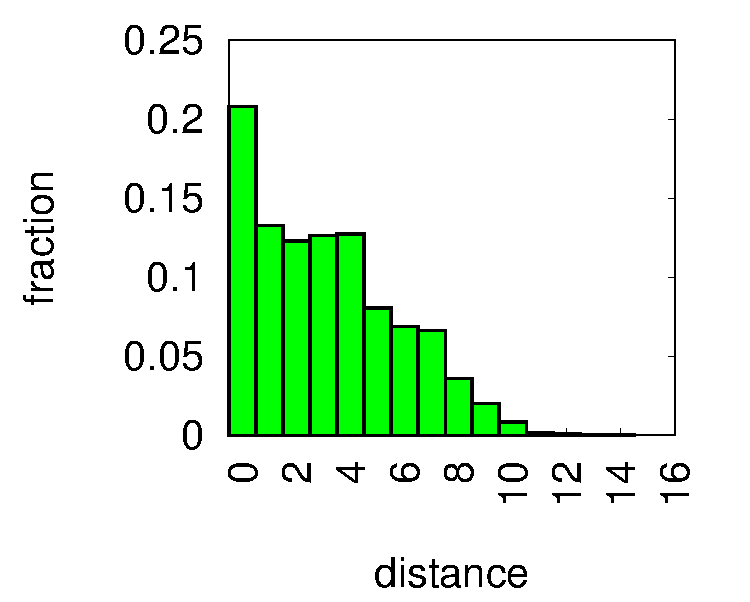
\includegraphics[width=0.3\textwidth]{/Users/owodo/MINE/PROJECTS/GraSPI/GraSPI/examples/2phaseMorphologies/thinFilm/histograms/data_0.615_4.0_000160.txtHistogramPolymerToInterface.pdf} \ ~ \ }
\parbox{0.3\textwidth}{\centering Tortuosity of D-paths to An  \newline
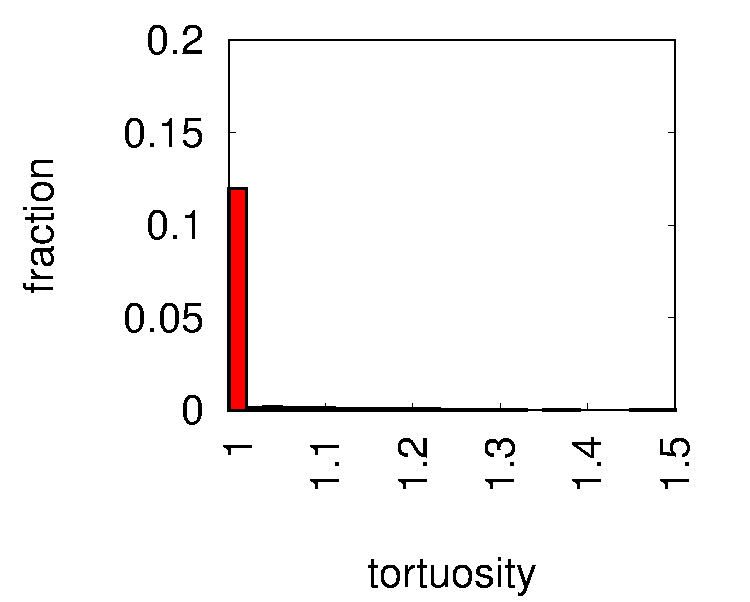
\includegraphics[width=0.3\textwidth]{/Users/owodo/MINE/PROJECTS/GraSPI/GraSPI/examples/2phaseMorphologies/thinFilm/histograms/data_0.615_4.0_000160.txtHistogramTortuosityPolymerToAnode.pdf} \ ~ \ }
\parbox{0.3\textwidth}{\centering Tortuosity of A-paths to Ca \newline
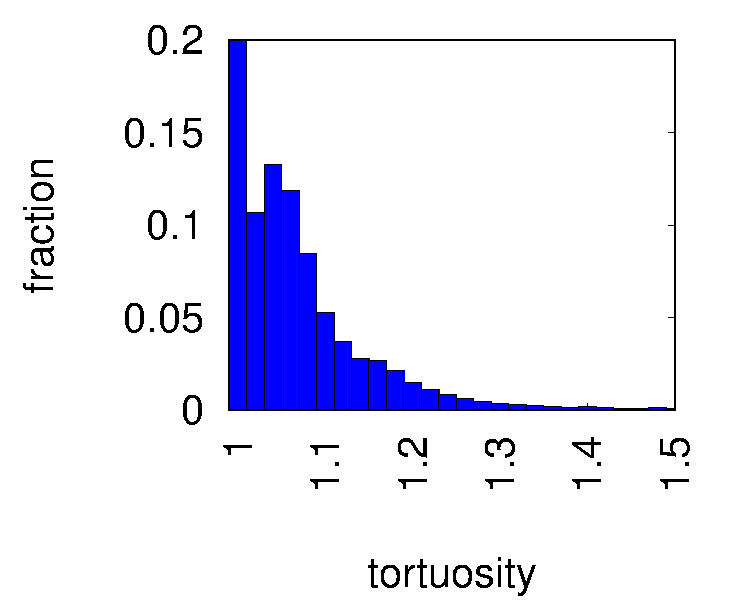
\includegraphics[width=0.3\textwidth]{/Users/owodo/MINE/PROJECTS/GraSPI/GraSPI/examples/2phaseMorphologies/thinFilm/histograms/data_0.615_4.0_000160.txtHistogramTortuosityFullereneToCathode.pdf} \ ~ \ }
}
\newpage
\end{document}
